\documentclass[10pt,twocolumn,letterpaper]{article}

% \usepackage{cvpr}              % To produce the CAMERA-READY version
\usepackage[pagenumbers]{cvpr} % To force page numbers, e.g. for an arXiv version

% Include other packages here, before hyperref.
\usepackage{graphicx}
\usepackage{comment}
\usepackage{amsmath}
\usepackage{amssymb}
\usepackage{booktabs}
\usepackage[toc,acronym]{glossaries}
\newacronym{AI}{AI}{Artificial Intelligence}
\newacronym{APC}{APC}{Autoregressive Predictive Coding}
\newacronym{CLI}{CLI}{Console Line Interface}
\newacronym{DL}{DL}{Deep Learning}
\newacronym{DQN}{DQN}{Deep Q Network}
\newacronym{DRL}{DRL}{Deep Reinforcement Learning}
\newacronym{GMM}{GMM}{Gaussian Mixture Models}
\newacronym{GPU}{GPU}{Graphical Processing Unit}
\newacronym{HPC}{HPC}{High Performance Computing}
\newacronym{InfoNCE}{InfoNCE}{Information Noise-Contrastive Estimation}
\newacronym{LSCC}{LSCC}{Lung Squamous Cell Carcinoma}
\newacronym{MOCO}{MOCO}{Momentum Contrast for Unsupervised Visual Representation Learning}
\newacronym{NLDL}{NLDL}{Northern Lights Deep Learning}
\newacronym{NLP}{NLP}{Natural Language Processing}
\newacronym{NRIS}{NRIS}{Norwegian Research Infrastructure Services}
\newacronym{RL}{RL}{Reinforcement Learning}
\newacronym{SSL}{SSL}{Self-Supervised Learning}
\newacronym{TCGA}{TCGA}{The Cancer Genome Atlas}
\newacronym{TD}{TD}{Temporal Difference}
\newacronym{UMAP}{UMAP}{Uniform Manifold Approximation and Projection}
\newacronym{WSI}{WSI}{Whole Slide Image}
\newacronym{XAI}{XAI}{Explainable AI}
\newacronym{tf-idf}{tf-idf}{term frequency-inverse document frequency}
\newacronym{CDR}{CDR}{Clinical Data Resource}
\newacronym{CPTAC}{CPTAC}{Clinical Proteomic Tumor Analysis Consortium}


\usepackage[pagebackref,breaklinks,colorlinks]{hyperref}
\usepackage[capitalize]{cleveref}
\crefname{section}{Sec.}{Secs.}
\Crefname{section}{Section}{Sections}
\Crefname{table}{Table}{Tables}
\crefname{table}{Tab.}{Tabs.}

\def\cvprPaperID{*****}
\def\confName{NLDL}
\def\confYear{2023}

% TODO Cite presentations?

\begin{comment}
The report should include both a short summary of the material covered (approx. 4 pages) and a description of the solution to a practical component.

Remember that the first four pages of your final report should cover aspects from all tutorials (not only focusing on the one relevant for the practical task)

Topics covered:
A gentle introduction to Deep Reinforcement Learning

Self-Supervised Learning: Training Targets and Loss Functions

The Challenge of Unverfiability in eXplainable AI Evaluation

Data representativity and low-resource modeling in deep learning

High Performance Computing for Deep Learning

Representation learning and learning with few data

\end{comment}

% if lacking text, write about the presentors (https://www.nldl.org/winter-school)

\begin{document}
\title{NLDL Winter School 2023}

\author{Anders Sildnes\\
University of Tromsø\\
Postboks 6050 Langnes\\
{\tt\small anders.sildnes@uit.no}
}
\maketitle
% Computational pathology is study of disease using methods such as artificial intelligence. For building models, there are three main hindrances: 1) lack of publicly available data, 2) large image-size and high number of details and 3) lack of ground truth data due to expert disagreeance. Consequently, developers have to compromise when building a model. To know if models are accurate enough, explainable AI can help. But, are the explanations good enough that a pathologist can trust a model used to evaluate patient diagnosis and/or prognosis? 


\section{Introduction}
\label{sec:intro}
This is a report from the 2023 Northern Lights Deep Learning (NLDL) conference. The first four pages contains a summary from each of the topics covered Monday 9th of January and Friday 13th January. A detailed programme can be found on the website: https://www.nldl.org/winter-school. Not all presentations could fully be summarized due to the length requirements, but I have chosen the topics I found most interesting.
% To make the first four pages I have followed each of the presentation slides and supplemented with extra information found in other sources, which of course are cited.
% if need be, summarize my findings here

\section{Deep Reinforcement Learning}
\begin{comment}
  \gls{RL} has emerged as a powerful technique in modern machine learning, allowing a system to learn through trial and error. We will introduce some fundamental principles upon which this family of methods is based. In the first part, we give a summary of classical reinforcement learning and thus provide the essentials for understanding Deep Reinforcement Learning (DRL). In the second part, we shift the focus onto DRL and look at how deep learning enhances classical reinforcement learning, leading to powerful new algorithms. These algorithms include DQN playing Atari games at a superhuman level, PPO solving robot locomotion problems, and Alpha Zero learning to play GO, Chess, and Shogi. In the limited time of such a mini-tutorial, we can of course only sketch the main characteristics, but we intend to motivate to look deeper into this fascinating family of methods.
\end{comment}
\gls{RL} is a branch of AI. One or more agents interact with a given environment and teach themselves 
behaviours that maximize a goal-function. Often this relies a great number of iterations; e.g. AlphaGo Zero played 4.9 million rounds of Go with itself before being released~\cite{goWithoutHumans}. This got news coverage all over the world as Go had long been considered to be a game too complicated for computers.

\gls{RL} agents operates in discrete time. At each timestep $t$ the agent observes its environment. Each observation $O_{t}$ modifies the agent state $s_{t}$, a processed representation to the history of events. Based on $s_{t}$ the agent chooses it's action $A_{t}$. The choice is made by choosing the action thought to maximize the reward $R_{t}$ of the agent in the future (next state). The expected return from the eyes of an agent is measured by it's goal function $G_{t}$, being the sum $G_{t} = \sum_{k=t+1}^{\inf{}}{R_{k}}$.
A problem with this goal function is that the agent can get stuck. E.g. in a dead end of a labyrinth; refusing to take a step back to find another path to the goal. A discount factor, noted $\gamma{}$, ensures that rewards less valuable over time, typically modelled as $G_{t} = \sum_{k=t+1}^{\inf{}}\gamma^{k}{R_{k}}$ (which can also be expressed a recursive $R_{t+1} + \gamma{G_{t+1}}$). Hence, if you stick in a dead end for too long, it doesn't pay off, and any other path that penultimately gets to another reward faster is better. The use of discount factors in reward functions is referred to as \textit{\gls{TD} learning}

But how is the reward chosen? Each state is given a \textit{value function}. This is the expected value from being in a state $s$: $V_{\pi} = \mathbb{E}_{\pi} [ G_{t} | s = s_{t}]$. $\pi$ is here defined as the policy for what action to choose. Usually we cannot know exactly what the outcome of an action is, therefore we model actions by stochastic policies $\pi{}(a | s)$ which gives likelyhood of future actions. An example is a robot taking a step forward, but sliding on a banana peel and consequently falling. This lesson means that re-visiting the same state later in the future should not yield the same action, even if the policy is the same. The same does not apply to e.g. chess, where we can set a deterministic policy since we know exact outcomes from actions (moving pieces). 
Analogous to the value function is the action value: $q_{\pi{}} = \mathbb{E} [ G_{t} \vert{} S_{t} = s \cap A_{t} = a]$. This function (as given here) is strict to the policy $\pi$, i.e., in order to predict the future value of actions, you have to stay with the same $\pi$. The \textit{q} is often referred to as \textit{quality}. 


% To resolve which future state that is desirable, the Bellman equation~\cite{bellman} is often used.
% It sums over all possible state successor states $s'$ and evaluates their estimated values given policy $\pi{}$ and probabilistic expection $p(s', r \vert{} s, a)$. It's full formal notation is given in~\Cref{eq:bellman}:
% \begin{equation}\label{eq:bellman}
%   V_{\pi}(s) = \sum_{a}{\pi(a\vert{}s})\sum_{s'}\sum_{r}{p(s', r \vert{} s, a) * [r + \gamma * v_{\pi{}}(s')]}
% \end{equation}

Keeping a mapping between states and their expected values can be exhaustive for computer memory. Finding the right policy can also be difficult. If we think of neural network for what they are, \textit{function approximators}, it seems intuitive to use them for approximating the value function and/or action policy. This helps us resolve the problem of finite available space in action-value mappings. Hence, the field of \textbf{\gls{DRL}} emerges. There are several examples already of popular tools/models built with \gls{DRL}, such as AlphaTensor CITE ,Stratego CITE, etc. 

The neural nets in \gls{DRL} (\gls{DQN}) lacks ground truth, but rather rely on rewards for optimization. The problem is that these rewards may come at delayed moments or at the influence of unknown variables. This is essentially noise in the learning loop. Therefore, there are several techniques used in conjuction with the neural nets to improve their accuracy. One such trick is experience replay: steps are recorded with $(s_{t}, a_{t}, s_{t+1}, r_{t})$ in a replay buffer. Now, whenever we perform an action, we can learn not only from the change in environment, but we may use extra samples from past events.

Talk more about policy gradients?

So far in this summary the \gls{RL} approaches have been \textit{model-free}: to learn of the world, actions are performed and evaluated. The alternative is \textit{model-based} \gls{RL}, wherein the agent can plan ahead by making predictions about how actions affect the world: $p(s_{t+1} \vert{} s_{t}, a_{t})$. The advantage of model-based \gls{RL} is primarily it's sample efficiency since we can prune away more actions during the learning phase. This is the case of Alpha Zero CITE. There have, however, been other strides in e.g. MuZero CITE, which can also train its own model to be used by \gls{RL} to predict future actions.

% The bellman equation is commonly used to asses a state value.

% This is often a greedy process where short-term benefits are prioritized over long-term benefits, similar to laws of finance, future gains are discounted. 


% \gls{RL} is sequential, i.e. future actions depend on previous ones. Unlike 


% TODO: Ai gyms?

\section{Self Supervised Learning}

\section{Unverfiability in eXplainable AI Evaluation}

\section{Data representativity and low-resource in Deep Learning}
\begin{comment}
This tutorial first introduces data representativity in artificial intelligence and machine learning, in particular how to measure data representativity and construct datasets that are fair and unbiased in contrast to datasets that work best on average. Secondly, we look at semi-supervised learning and transfer learning for low-resource applications, including a variational autoencoder for speech. The two parts consider robustness towards distribution shifts from a data and a modelling perspective.
\end{comment}
\gls{DL} depends on many iterations with data to improve its accuracy. If there are biases in the training data, this will also affect the inference results. We are therefore quite keen on getting \textit{representative samples} for our model training. But the term representative is ambigious and that in this ambiguity there are many research projects that fallaciously claim that their model is general. As a sidenote, it is also important to remember that we sometimes do not want our model to only work well in general cases. A medical scanner should work just as well for a representative user as any other user. E.g. most hearth disease occurs in elderly, but scanners should work well on children, too, unless you build another machine for non-specific usecases.

CITE Kruskal
According to there are 6 notions that are used to claim representativity.
The first is \textbf{assertive claims}, which state that they have general or all-covering data without explaining why. One might say that since ImageNet CITE has many photos, it is general, but this has been found to not be the case CITE.
Second, there is \textbf{``the miniature''}, wherein sub-populations might be over- or undersampled. These miniature models may suffer from a poor choice of stratifying attributes, either from misconceptions or subjective biases of the sampling author.
Third, there is \textbf{absence or presence of selective forces}. A survey will never measure non-responsders for example (``selection force'') and a random sample may not be representative if e.g. the sampling phase is chosen poorly (``absence of selective forces'').
Forth, there is the \textbf{Typical/Ideal} sample, wherein samples used are supposedly averages of their subgroup. One example is choosing cluster centers from Gaussian Mixture Models.
Fifth, there is \textbf{Coverage Claims}. In a ``Noah's Ark-esque'' fashion, subgroups of data are sampled in equal numbers so as to avoid the potential of other biases. There are pitfalls here too, however, such as not covering the entire data span. To do full coverage, it is often common to see both random and non-random sampling used together: selecting groups deliberately, but samples from that group randomly.
Sixth, there is a the deferral of defining representativity, giving instead a \textbf{reference to sampling methods}. The notion is carried by the idea that all datasets will \textit{always} be only a minitature model and subject to bias, so rather than claiming a \textit{definitive} data representativity, you leave it to the reader. 

\Cref{datarepresentativity} additionally defines two other notions particlarly relevant for \gls{AI}. The seventh notion is \textbf{the copycat}, where synthetic data is used to claim representativeness. Finally, the last notion is the simplest one: you do not talk about representativity at all. 

Assertive and ``no-notion''-claims are to be avoided in science. The rest may, however, be viable based on the context.

Talk about semi-supervised tranfser? ugh

\section{High Performance Computing for Deep Learning}
The \gls{NRIS} (formerly ``the Metacenter'') is a collaboration of multiple organisations in Norway to share experience and offer services and resources for research. One of these services are Sigma2, which offers a \gls{HPC} environment. The computers are stored both at NTNU and UiT.

\gls{HPC} are comprised of a large number of storage and processing units, allowing programmers to solve problems that are too big for consumer-level computers. Unlike another option, cloud environments, \gls{HPC} store all their resources in the same location and usually have shared file drives. This makes it fast to launch distributed workloads. There are two paradigm shifts according to CITE sigma2 that you need to overcome when using \gls{HPC}; 1) working with \gls{CLI} and 2) working with multiple computers. Additionaly, \gls{HPC} clusters are often in high demand, resulting in the need of job schedulers. 

In \gls{DL}, an immediate advantage of \gls{HPC} is the higher number of \gls{GPU} available, potentially removing the need for batch-processing. However, working with multiple \gls{GPU} introduces some challenges: how and when do we communicate between nodes? There's two primary modes: synchronous and asynchronous. Synchronous processing is often faster~\cite{distributedDL}, but may be bottlenecked by slower or interrupted machines. Furthermore, synchronization points may be costly (slow), leaving nodes idling. Asynchronous processing mitigates these problems, but have other costs. Many asynchronous frameworks will e.g. have smaller workloads per kernel, giving extra overhead to load balancers that have to distribute remaining work~\cite{pan2017synchronous}.

\section{Representation learning and learning with few data}

\section{Practical project}
\cite{sslUMAP} uses self-supervised learning to learn morphological features of Lung Squamous Cell Carcinoma (LSCC). In training they use public TCGA and CPTAC datasets of H\&E-stained biopsy slides. They observe from previous work that other training algorithms cluster together tiles from the same slides, creating a batch effect where the algorithm learns features that are more slide specific than feature specific. This indicates that the network might do poorly on generalized input. They visualize this using 2D UMAP, shown in~\cref{fig:umap}.

\begin{figure}
  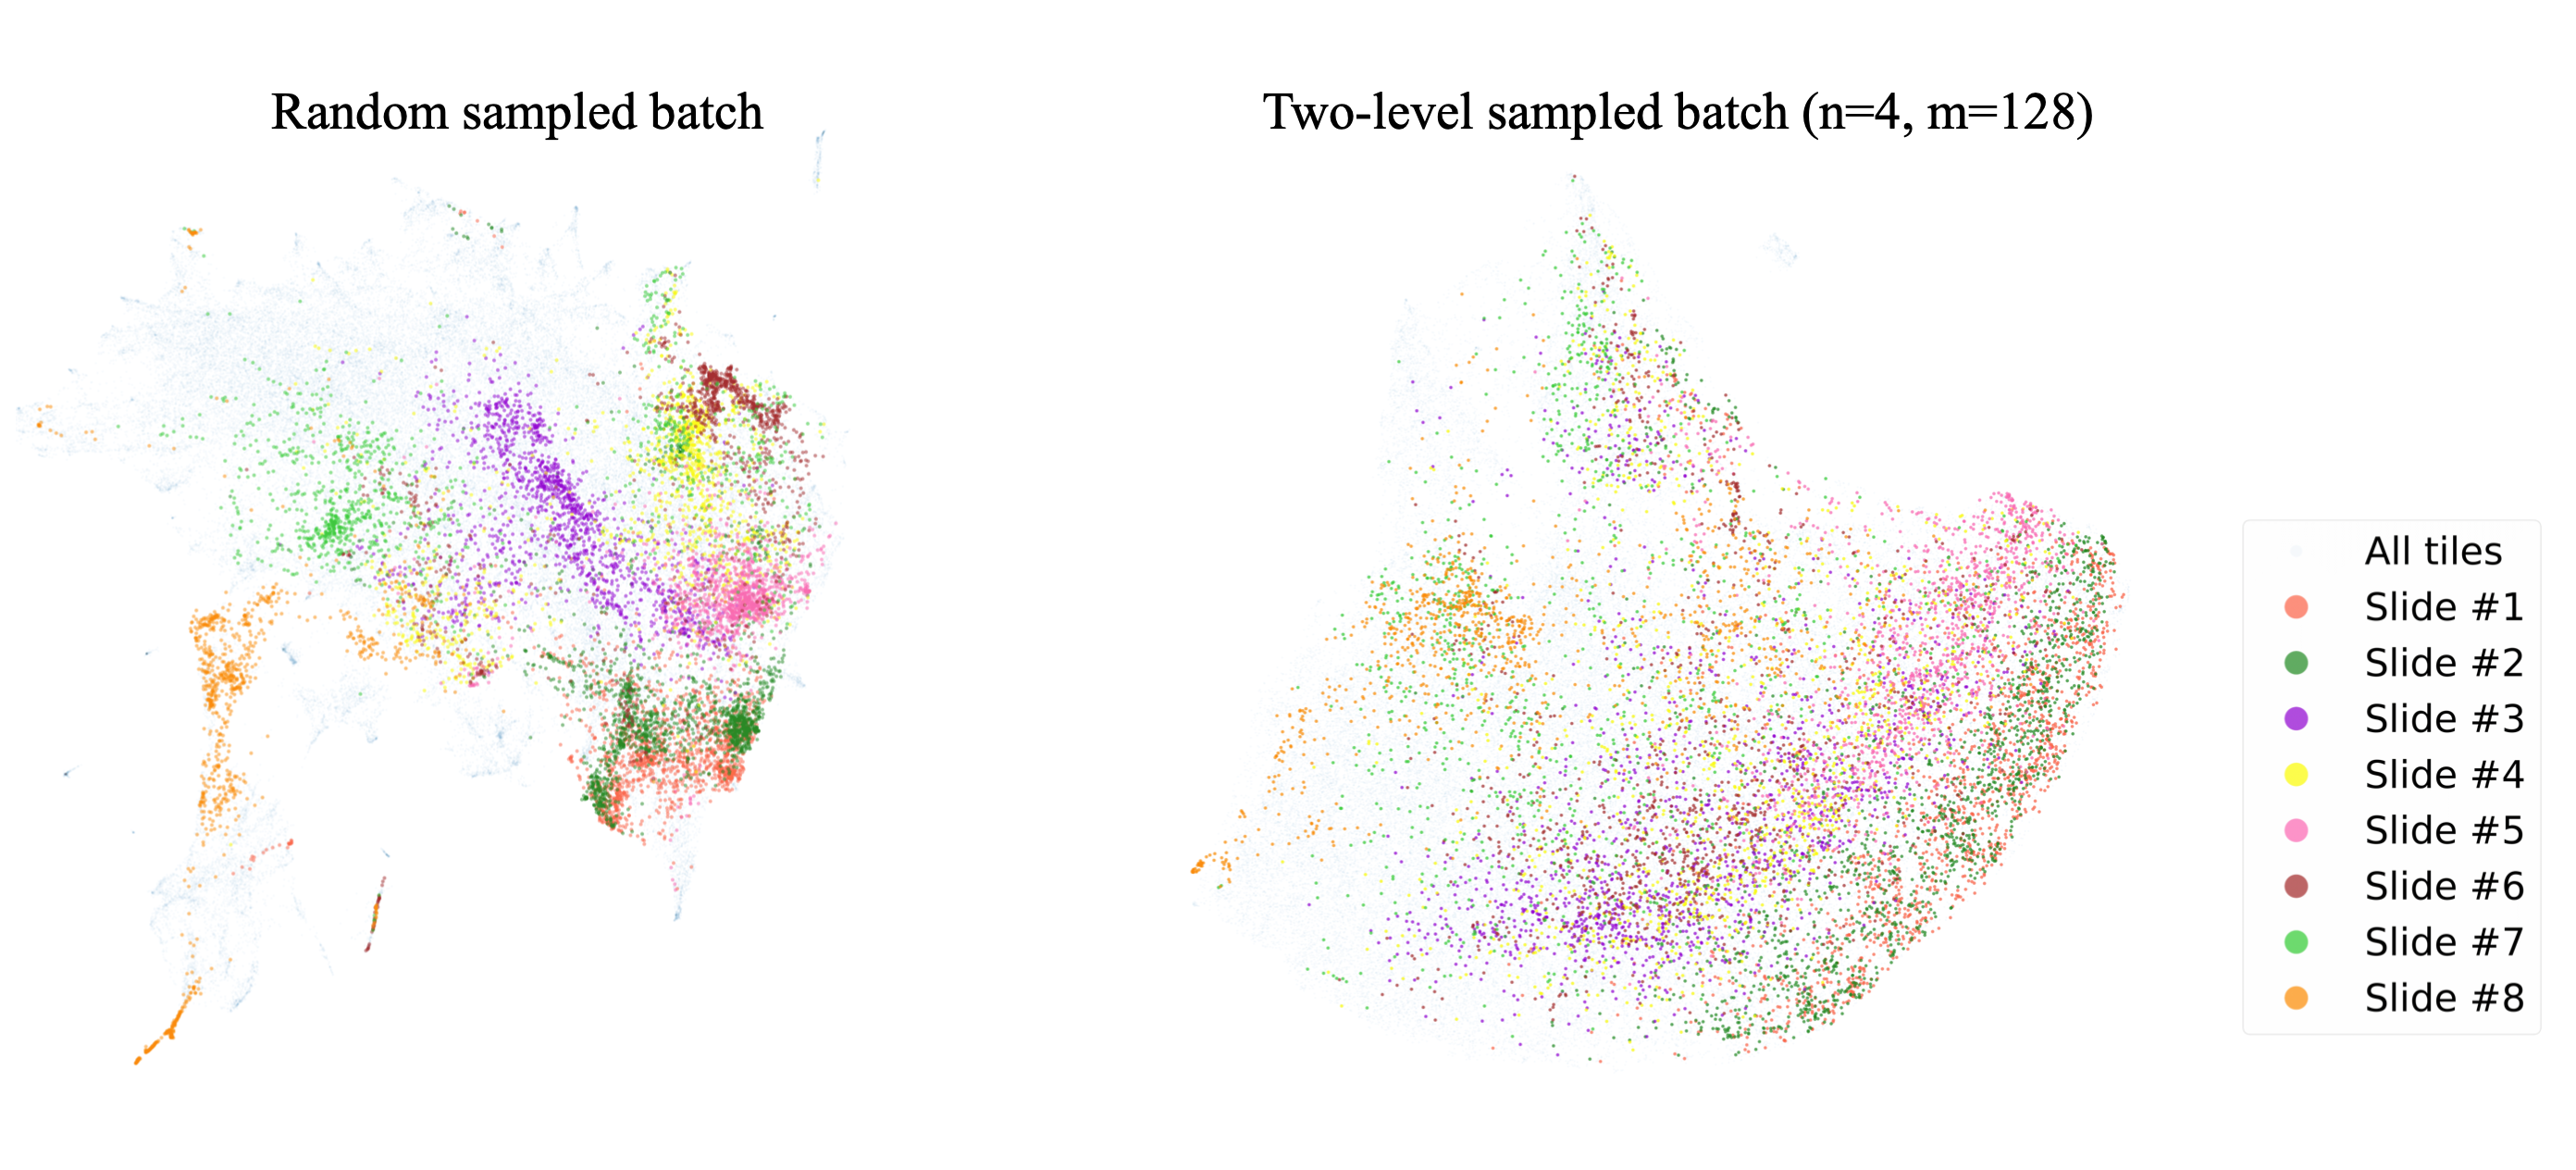
\includegraphics[scale=.17]{./umap.png}
  \caption{Figure taken entirely from~\cite{sslUMAP}. Both pictures show a 2D UMAP projection of tile representations. On the left a training algorithm with randomly sampled tiles from slides, showing that features learned in the same slide cluster together. Using a different sampling algorithm, the picture on the right shows a more even distribution w.r.t slides}
  \label{fig:umap}
\end{figure}

\subsection{UMAP}
 The algorithm is founded on three assumptions about the data
 \begin{enumerate}
   \item The data is uniformly distributed on Riemannian manifold;
   \item The Riemannian metric is locally constant (or can be approximated as such);
   \item The manifold is locally connected.
 \end{enumerate}

lack of ground truth in the data; I cannot say that two neighbors should be similar, since a model may model two samples differently even if the samples themselves are similar.

A good scoring method can indicate for each slide whether there is overlap with others; this slides is probably overfitted
A good scoring method can also average, though.
Have to keep in mind that two photos can be disparate, e.g. 1 photo can have tumours, the other can be healthy, e.g.

TODOØ 2.9.1 Reflection in Clemmensen has a lot of stuff about metrics.


I wish to evaluate~\cite{sslUMAP} and quantify the quality of \textit{the explanation} using metrics inspired by Quantus~\cite{hedstrom2022quantus}. This means 1) finding relevant qualitative metrics for the given batch effect plots and 2) testing how the metrics change with model, batch and image adjustments. In particular, I am curious how well the metrics show batch/clustering effects for few (1-3) slides. This can be a useful indication early during a training process.

%%%%%%%%% REFERENCES
{\small
\bibliographystyle{ieee_fullname}
\bibliography{egbib}
}

\end{document}
